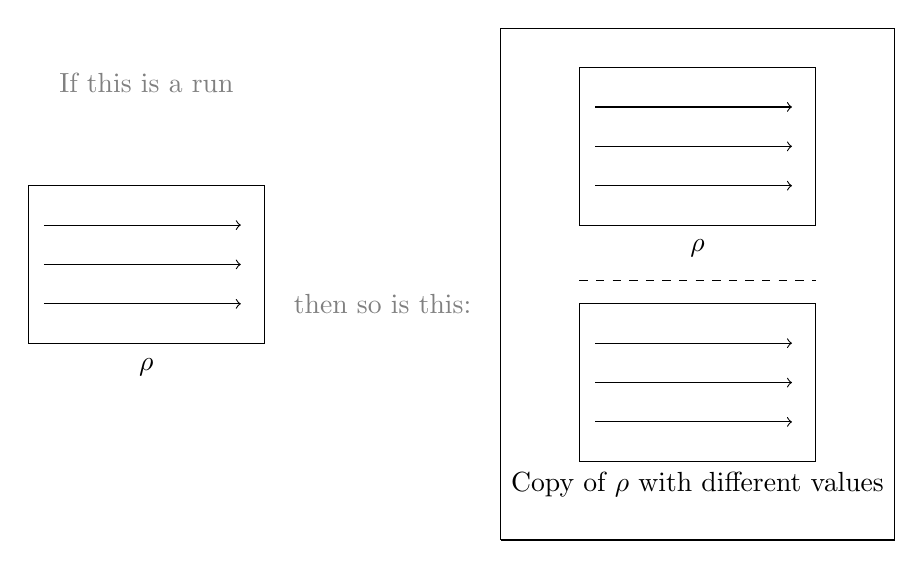
\begin{tikzpicture}
	
	
	
	\draw (0, 0) -- (3, 0) -- (3,2) -- (0,2) -- (0,0); 
	
	\draw (7, 1.5) -- (10, 1.5)  -- (10,3.5) -- (7,3.5) -- (7,1.5); 
	
	\draw (7, -1.5) -- (10, -1.5) -- (10,0.5) -- (7,0.5) -- (7,-1.5); 
	
	\draw (6, -2.5) -- (11, -2.5) -- (11,4) -- (6,4) -- (6,-2.5); 
	
	\node[color=gray] (r) at (1.5, 3.3) {If this is a run};
	\node[color=gray] (r) at (4.5,0.5) {then so is this:};
	
	
	
	\node (r) at (1.5,-0.3) {\normalsize$\rho$};
	\node (r1) at (8.5,1.2) {\normalsize$\rho$};
	
	\draw[dashed] (7,0.8) -- (10,0.8);
	
	\node (r2) at (8.5,-1.8) {Copy of \normalsize$\rho$ with different values};
	
	\draw[->] (0.2, 1.5) -- (2.7, 1.5);
	\draw[->] (0.2, 1) -- (2.7, 1);
	\draw[->] (0.2, 0.5) -- (2.7, 0.5);

	\draw[->] (7.2, 3) -- (9.7, 3);
	\draw[->] (7.2, 2.5) -- (9.7, 2.5);
	\draw[->] (7.2, 2) -- (9.7, 2);
	
	\draw[->] (7.2, 0) -- (9.7, 0);
	\draw[->] (7.2, -0.5) -- (9.7, -0.5);
	\draw[->] (7.2, -1) -- (9.7, -1);
	
\end{tikzpicture}